\chapter{Prolog}
\label{sec:Prolog}
In Prolog dreht sich alles um das erstellen von Wissensbasen und deren Auswertung. Fakten und Regeln zusammen ergeben eine Wissensbasis und sind zusammen mit Anfragen die 3 Konstrukte aus denen sich diese Sprache zusammensetzt. Regeln und Fakten gehören und zu den Prädikaten. Fakten können weiterhin unterteilt werden in Funktoren und Atome. Dazu das passendes Bild. 

\begin{figure}[h]
\centering
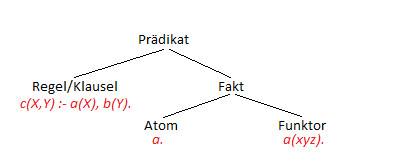
\includegraphics[width=0.5\linewidth]{mainmatter/pics/Prolog}
\caption[Prädikat Unterteilung]{Prädikat Unterteilung}
\label{fig:Prolog}
\end{figure}

\subsection{Atome}
\begin{itemize}
	\item fängt mit einem a-z
	\item bestehen aus den Zeichen a-z, A-Z, 0-9, \_
	\item Ein String in ' ' .z.B. 'Hi', auch als Name des Atoms bezeichnet. Leerzeichen sind innerhalb dieser Anführungszeichen erlaubt.
	\item Spezielle Zeichenketten sind erlaubt. Diese sind:
	\begin{enumerate}
		\item @= oder == oder ; oder :-  . Jedoch fallen ; und :- Sonderrollen zu. Mit ; fragt man nach weiteren Antworten von dem Programm und :- gehört fest zu einer Regel.
	\end{enumerate}
\end{itemize}
Hinweis: YAP und andere Prolog Interpreter erkennen 'mia' = mia. An und geben Yes aus. Jedoch '2' = 2. wird immer mit einem No konfrontiert. 
\subsection{Variablen}
\begin{itemize}
	\item Variablen beginnen mit A-Z oder \_ 
	\item bestehen aus den Zeichen a-z, A-Z, 0-9, \_
\end{itemize}
\section{Notation}
Im Nachfolgenden gibt es einen kleinen Überblick über die Notationen in Prolog.
\subsection{Und / Oder in Regeln}\qquad\\
, $\Leftrightarrow$ Und\\
; $\Leftrightarrow$ Oder
\subsection{Numerische Vergleichsoperatoren:}\qquad\\
\begin{align*}
\text{X }   &=:=  \text{  Y    numerisch gleich}\\
\text{X }  &=\backslash= \text{  Y    numerisch ungleich}\\
\text{X }   &<\text{   Y    X kleiner als Y}\\
\text{X }   &>\text{   Y    X größer als Y}\\
\text{X }  &=<\text{   Y    X kleiner gleich Y}\\
\text{X }  &>= \text{  Y    X größer gleich Y}\\
\end{align*}
!! Bei Vergleichen müssen alle Variablen belegt sein.



\subsection{Numerischer Auswertungsoperator:}\qquad\\
Ein einfaches Beispiel um X Berechnete Werte zu übergeben. \\
X is 6+3.\\
Achtung, wenn man X is Y + Z. schreibt, müssen Y und Z bereits belegt sein. Ansonsten führt dies zu einem Error. 

\subsection{Term-Vergleichsoperatoren:}\qquad\\
\begin{align*}
\text{X }   &=   \text{ Y    unifizierbar}\\
\text{X }  &\backslash=   \text{ Y    nicht unifizierbar}\\
\text{X }  &==   \text{ Y    identisch mit}\\
\text{X }  &\backslash== \text{ Y    nicht identisch mit}\\
\end{align*}




\subsection{Numerische Operatoren}

+     Addition

-     Subtraktion

*     Multiplikation

/     Division    

//    Ganzahl-Division

**    Potenz

mod   Modulo

/$\backslash$    bit-weises UND   (\& in C und C++)

$\backslash$/    bit-weises ODER  (| in C und C++)


\subsection{Typtest}\qquad\\
Dies dient zur Bestimmung des Types der einzelnen Atome.\\
atom/1 	Is the argument an atom?\\
integer/1 	Is the argument an integer?\\
float/1 	Is the argument a floating point number?\\
number/1 	Is the argument an integer or a floating point number?\\
atomic/1 	Is the argument a constant? no var, or term. \\
var/1 	Is the argument an uninstantiated variable?\\
nonvar/1 	Is the argument an instantiated variable or another term that is not an un instantiated variable? \\
Dabei gilt besonders folgendes zu beachten bei dem Test auf atom. \\

\begin{lstlisting}[language=Prolog] 
Erst instanziert dann getestet. 
?-  X  =  a,  atom(X).
X  =  a
yes

Erst getestet dann instanziert. 
?-  atom(X),  X  =  a.
no 
\end{lstlisting}
\section{Wissensbasis}\qquad\\
Als Wissensbasis bezeichnet man eine Zusammenstellung von Fakten und Regeln. Im folgenden Beispiel ist alles vorhanden. 
\begin{lstlisting}[language=Prolog] 
happy(yolanda).
listens2Music(mia).
listens2Music(yolanda):-  happy(yolanda).
playsAirGuitar(X):-  listens2Music(X). 
\end{lstlisting}
Es gibt insgesamt 2 Fakten in dieser Wissensbasis. happy(yolanda) und listen2Music(mia). Diese Fakten werden auch Funktore genannt, da diese ein Atom einklammern. Ein Reiner Fakt würde z.B. yolanda sein. \\
Die letzten Beiden Zeilen in diesem Beispiel sind Regeln. diese Zeichnen sich durch :- aus und können auch Variable gehalten werden. Die erste Regel (listens2Music(yolanda):-  happy(yolanda).) wird per Pattern Matching (siehe dazu auch das Pattern Matching in Haskell$^{\ref{sec:hpm}}$) lediglich auf die Anfrage\\ ?-listen2Music(yolanda) reagieren. Alle anderen Fälle fängt die zweite Regel ab. Hier werden die Eingaben, mit X Unifiziert$^{\ref{sec:unifikation}}$. \\
Die Regel splittet sich in einen Kopf und einen Körper auf. Alles was vor dem :- steht ist der Kopf und alles was danach steht ist der Körper. 
\section{Rekursionen}\qquad\\
Auch in Prolog gibt es Rekursionen und diese werden stark genutzt. Damit können zum Beispiel Listen durchgearbeitet werden um zu schauen, wie lange eine Liste ist. Listen könen hier beliebige Datentypen enthalten und sind nicht Typisiert wie in Haskell. 
\begin{lstlisting}[language=Prolog] 
len([],0) .
len([_|T],N):-len(T,X) ,N is X + 1.

Aufruf:
?- len([1,2,3,4],X).

Ergebnis:
X = 4?
yes
\end{lstlisting}
Nehmen wir diese Rekursion einmal auseinander.\\
Die erste Zeile in diesem Beispiel ist die Abbruch Bedingung. Diese wird wahr, wenn die Liste leer ist und definiert die Länge der leeren Liste als 0. Zu dieser 0 wird jeweils durch Backtracking, dem zurück schreiten im Lösungsbaum, eine eins hinzu addiert. Dies ergibt die Länge der Liste. \\
\qquad\\
Es ist \textbf{extrem wichtig}, dass die Abbruchbedingung als erste bei einer Rekursion genannt wird. Denn Prolog arbeitet von oben nach unten. Wenn wir zuerst die Rekursion (Zeile 2) geschrieben hätten würde dies zu einem Fehler führen. \\
Beginne bei einer Rekursion immer zuerst mit der Abbruchbedingung, und stelle den rekursiven Aufruf so weit wie möglich ans Ende der rekursiven Regel.
\section{Unifikation}\label{sec:unifikation}\qquad\\
Das Ergebnis einer Unifikation ist eine Liste von Variablenersetzungen, die man vornehmen muss, um zwei Ausdrücke identisch zu machen. Diese Liste ist zustandsfrei (für alle Zeiten gleich und unveränderlich).\\ Prolog legt im Hintergrund jede Variable nach einem bestimmten Muster an. Dieses Muster ist \_5874 Wobei die Zahlen abweichen können. 
\begin{lstlisting}[language=Prolog] 
Beispiel 1:
eats(fred,tomatoes).
eats(Whom,What) .

Beispiel 2:
likes(jane,X).
likes(X,jim).

Beispiel 3:
f(foo,L).
f(A1,A1).

Beispiel 4:
X = t(X).
\end{lstlisting}
\textbf{Lösungen:}\qquad\\
\begin{enumerate}
	\item Unifikation ist möglich da Whom = fred und What = tomatoes. Bis hier hin keine große Verwunderung.
	\item Unifikation ist \textbf{nicht} möglich da X nicht gleichzeitig zwei Werten zugeordnet werden kann.
	\item Unifikation ist möglich. Denn A1 wird mit foo unifiziert und da L auch eine Variable ist, kann diese auch mit A1 und somit mit foo unifiziert werden. 
	\item Unifikation wird endlos weiter geführt. Denn X = t(X) = t(t(X)) \dots
\end{enumerate}


\section{Resolution}

\section{Akkumulatoren}
\section{Cut}
\section{Status}